\subsection{Аналитический обзор литературных источников}
\label{sec:analysis:literature}

Далее приводится анализ сведений, которые влияют на формулирование требований, дальнейшее проектирование и разработку программного средства.

\subsubsection{} Обзор основных составляющих персонального бюджета
\label{sec:analysis:literature:components}

Бюджет -- это документ (электронный или бумажный), в котором регулярно, наглядно и детально отображаются все статьи доходов и расходов за конкретный период времени, другими словами -- все источники притока средств, все траты, а также какие-либо индивидуальные правила распоряжения финансами и личный финансовый план на будущее~\cite{budget_blog}.

Ведение персонального бюджета включает в себя несколько базовых частей, которые со временем дополняются другими, приобретая черты более сложной системы.
Основными компонентами ведения личного бюджета являются:
\begin{itemize}
    \item учёт доходов и расходов;
    \item оптимизация расходов;
    \item планирование доходов и расходов.
\end{itemize}

Стоит отметить, что каждый последующий компонент является логическим продолжением предыдущего.

В прикладном прогнозировании нередко возникают ситуации, когда математическое моделирование, основанное на использовании точных законов, оказывается затруднительным, но в распоряжении исследователей оказывается выборка прецедентов -- результатов наблюдений исследуемого процесса или явления, включающих значения прогнозируемой величины~\cite{prediction_basics}.
Так как каждый человек распоряжается деньгами уникальным образом, то получение точных законов по планированию расходов практически невозможно.
Поэтому \emph{учёт доходов и расходов} является необходимым и основным компонентом учёта персонального бюджета.
Данный компонент отвечает за получение исторических и текущих данных о расходах, которые можно будет использовать в планировании и оптимизации.
Учёт доходов необходим для того чтобы точно определить конкретные источники доходов, их регулярность и величину.
В то же время учёт расходов более важен, так как позволяет определить конкретные категории денежных потоков, какие из них являются необходимыми, а какие можно ограничить или убрать вовсе.

\emph{Оптимизация расходов} подразумевает рациональное использование средств.
Основной целью данного этапа является выявление наиболее убыточных категорий, отсутствие трат на которые незначительно изменит общий уровень жизни. Также в рамках данного этапа необходимо выделить \emph{обязательные} и \emph{необязательные} категории расходов.
Например, категорию <<коммунальные услуги>> можно отнести к первому типу, а <<кино>> -- ко второму.
Оптимизация расходов в основном направлена на необязательные категории расходов, так как они зачастую непостоянны и напрямую зависят от желаний и самоконтроля человека.

Расходы на обязательные категории трудно сократить, так как зачастую человек не может прямым образом влиять на их размер: ставки на электроэнергию и водоснабжение устанавливаются внешними структурами.
При этом данный тип категорий легко поддается планированию, так как эти суммы достаточно постоянны.

Любое планирование -- это существенная составляющая успеха в любой сфере жизни, так как позволяет не только разделить процесс достижения цели на несколько важных этапов, но и увидеть новые возможности.

\emph{Финансовое планирование} -- выбор целей по реальности их достижения с имеющимися финансовыми ресурсами в зависимости от внешних условий и согласование будущих финансовых потоков. Выражается в составлении и контроле над выполнением планов формирования доходов и расходов, учитывающих текущее финансовое состояние, выраженные в денежном эквиваленте цели и средства их достижения~\cite{finance_planning}.

Все планы, в том числе и финансовые, подразделяются, как правило, на краткосрочные (до 1 года), среднесрочные (от 1 года до 3 лет) и долгосрочные (от 3 лет и более).
Для наилучшего результата рекомендуется планировать начиная с краткосрочных планов.
Во-первых, достижение целей -- это процесс поэтапный, в котором реализация среднесрочных или долгосрочных планов может зависеть от краткосрочных или среднесрочных.
И, во-вторых, всегда существует определенный рубеж, преодолеть который в конкретный момент человек не может.
К тому же, имеют место быть некоторые обстоятельства, повлиять на которые достаточно сложно.
К таким обстоятельствам можно отнести инфляцию, внезапное сокращение на работе, непредвиденные необходимые траты и прочее.
Чтобы иметь возможность быть готовым, если не ко всему, то ко многому, требуется иметь четкое представление о том, что делать в той или иной ситуации, а также разработать свою стратегию по достижению целей.
Всё это и включает в себя финансовое планирование.
Лучшим временем для приведения бюджета в порядок и планирования является начало года, однако это не является обязательным требованием.

Полученная информация поможет определить, на какие аспекты учёта персонального бюджета следует обратить повышенное внимание во время формирования требований к проектируемому средству.

\subsubsection{} Обзор подходов по учёту доходов и расходов
\label{sec:analysis:literature:tracking}

Как было упомянуто в пункте~\ref{sec:analysis:literature:components}, учёт доходов и расходов является базовым компонентом для качественного учёта персонального бюджета.
Существует множество разнообразных средств для реализации этой цели.
Независимо от того, какое средство будет задействовано, все они рассчитывают на точность введенных данных.

\emph{Бумажный метод} учёта доходов и расходов существует уже десятки лет и является одним из первых подходов для достижения финансовой стабильности.

В самом простом своём появлении данный метод требует только простого блокнота и ручки, куда записывают все траты по мере их поступления (см. рисунок~\ref{fig:analysis:literature:paper_log}), либо в конце дня по наличию чеков оплаты.
Существуют специальные бумажные издания с напечатанными таблицами, которые заполняют информацией о доходах.

\begin{figure}[H]
    \centering
    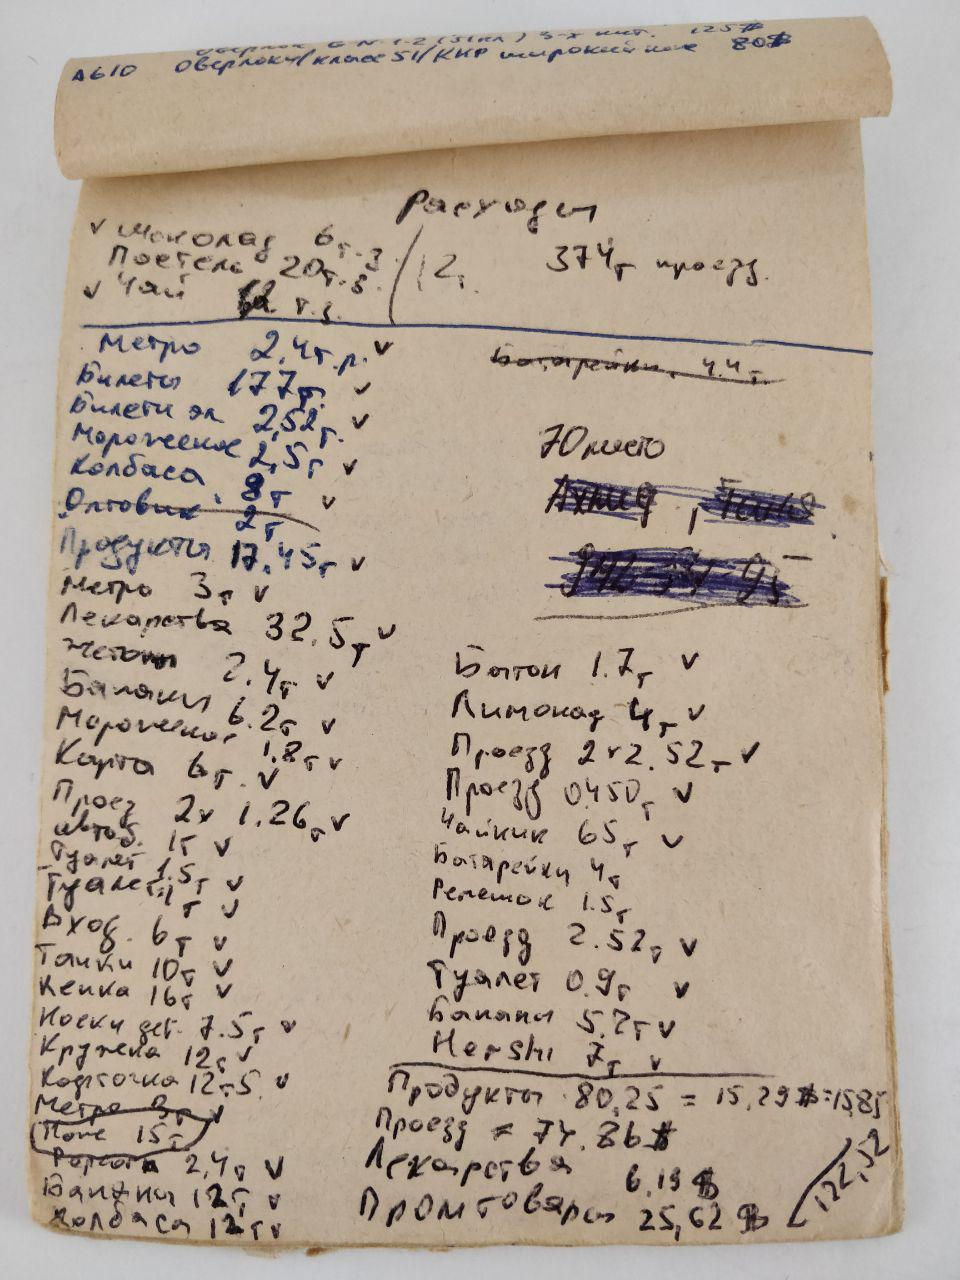
\includegraphics[scale=0.52]{1_1_2_paper_log.png}
    \caption{Пример ручного учёта расходов в блокноте}
    \label{fig:analysis:literature:paper_log}
\end{figure}

Однако бумажный метод является относительно устаревшим и имеет несколько недостатков, таких как необходимость постоянно носить упомянутый блокнот с собой, низкая скорость записи и изменения транзакций, необходимость подсчитывать суммы вручную.

С развитием информационных технологий появились различные решения с использованием вычислительной техники.
Одним из первых таких решений является использование программного обеспечения по работе с электронными таблицами, такими как \emph{Microsoft Excel} или \emph{Google Spreadsheets}.

Подобные программные решения упрощают занесение и редактирование новой информации, также имеются большие возможности по использованию встроенных формул и построения графиков.
Среди недостатков стоит выделить тот факт, что подобные системы в основном рассчитаны на использование с персонального компьютера, что сильно затрудняет своевременный ввод информации о транзакциях из-за того, что компьютер зачастую недоступен в момент совершения операций с деньгами.

Также существуют специализированные программные решения учёта доходов и расходов для различных платформ.
Среди них выделяют:
\begin{itemize}
    \item настольные приложения;
    \item мобильные приложения;
    \item веб-приложения.
\end{itemize}

\emph{Настольное приложение} -- программное средство, которое запускается локально на компьютере пользователя.
Такие приложения имеют богатую функциональность для решения задач по учёту доходов и расходов, планированию и отображению различных графиков и диаграмм.
Однако, как и ПО для работы с электронными таблицами, данный тип приложений зачастую не находится в быстром доступе.
Данного недостатка нет у \emph{мобильных приложений} -- в современном мире почти всегда люди имеют под рукой мобильное устройство.
Также появляется возможность использования мгновенных оповещений~\cite{desktop_mobile_differences} и интеграциями с другими особенностями мобильных устройств.
Но для таких приложений актуальны ограничения платформ, на которых они запускаются, такие как меньшие размеры экранов, более медленные процессоры, ограниченное время работы в автономном режиме.
\emph{Веб-приложения}, в отличие от настольных и мобильных, работают на удаленном аппаратном обеспечении и поставляются пользователю через браузер~\cite{web_based_vs_desktop}.
Это позволяет использовать его как с мобильного устройства, так и с персонального компьютера.
Помимо того, что существуют задержки при передаче, особенно при нестабильном соединении, сама потребность в постоянном интернет соединении может значительно снизить удобство пользования приложением.
Кроме того, размер загружаемого при каждом запуске кода и ресурсов может значительно увеличить траты пользователя, особенно если он использует дорогое мобильное подключение к интернету.

\subsubsection{} Обзор методик планирования бюджета
\label{sec:analysis:literature:planning}

Проблема учёта персонального бюджета существует уже многие годы.
За эти годы было выработано большое методик распределения заработанных ресурсов которые в разной степени контролируют распределение заработанных ресурсов.
Среди наиболее популярных следует выделить:
\begin{itemize}
    \item метод четырех конвертов;
    \item метод шести кувшинов;
    \item правило шестидесяти;
    \item система \emph{Kakebo}.
\end{itemize}

\emph{Метод четырех конвертов} основывается на чётком разделении трат на четыре недели с предварительным выделением определенной суммы на сбережения и регулярные расходы.
Данный метод рассчитан на людей с фиксированным регулярным ежемесячным доходом и подразумевает, что в месяце содержится приблизительно четыре недели.
Перед разделением денег на еженедельные конверты сначала откладывают десять процентов доходов для сберегательных целей, однако процент может быть и другим в зависимости от целей и финансовых возможностей.
Затем выделяют определенную сумму на регулярные известные платежи, те расходы, которые нужно совершать каждый месяц, и сумма их известна, и она обычно одинаковая или разнится, но несущественно~\cite{four_envelope_rule}.

К плюсам метода стоит отнести его простоту и лёгкость в организации.
Из минусов стоит отметить необходимость учитывать непредвиденные обстоятельства, такие как затраты на лечение или штрафы, а также потребность в учёте дополнительных дней в месяце, которые выходят за рамки четырех недель.

Также существует \emph{метод шести кувшинов}.
Суть метода кувшинов заключается в том, чтобы распределять все поступления в личный или семейный бюджет на 6 неравных частей (6 кувшинов), каждый из которых имеет свое строгое предназначение~\cite{six_jugs}.
Кувшины могут представляться как в виде конвертов с наличностью, так и в виде виртуальных счетов.
По правилам метода перекладывать деньги из кувшина в кувшин строго запрещается.
Определяются следующие типы кувшинов:
\begin{itemize}
    \item \emph{Необходимые нужды}, на которые распределяется 50\% всей суммы доходов, предназначен для постоянных, необходимых для обычной жизни категорий расходов, таких как еда, ипотечные платежи, счета и так далее.
    \item \emph{Финансовая независимость} -- 10\% общих доходов предназначены только для накоплений или инвестиций -- всего того, что повышает богатство и финансовую независимость в будущем.
    \item \emph{Большие покупки} -- 10\% доходов выделяется на покупки, которые человек не в состоянии оплатить из своих текущих трат, такие как машина, квартира и тому подобное.
    \item \emph{Обучение}, на которое выделяется 10\% общих доходов, назначается для трат на саморазвитие, так как автор метода шести кувшинов считает, что с увеличением знаний и навыков повышается и способность зарабатывать деньги.
    \item \emph{Развлечения} предполагают 10\% всех денег для трат на любые вещи, которые приносят удовольствие или <<прожигают деньги>>, так как метод предусматривает человеческий фактор и потребность людей тратить деньги спонтанно, без какой-либо причины.
    \item \emph{Подарки} -- 10\% общих доходов выделяется на подарки родным и близким, а также благотворительность.
\end{itemize}

Похожую методику придумал Ричард Дженкинс, которая называется \emph{правило 60\%}.
Она также основывается на разделении всего дохода на несколько неравных частей.
По данной методике предлагается разделить доход на пять частей:
\begin{itemize}
    \item 60\% -- текущие расходы;
    \item 10\% -- пенсионные накопления;
    \item 10\% -- долгосрочные покупки и выплаты;
    \item 10\% -- нерегулярные расходы;
    \item 10\% -- развлечения.
\end{itemize}

Текущие расходы в методике включают в себя следующие статьи расходов:
\begin{itemize}
    \item основные потребности в еде и одежде;
    \item существенные бытовые расходы;
    \item все счета, включая коммунальные услуги, интернет и другие;
\end{itemize}

Нерегулярными расходами являются траты, которые не входят в стандартные расходы, например, ремонт автомобиля, деньги на лечение или подарки.

Очень популярной методикой является \emph{kakebo} -- это система учета индивидуальных расходов, позволяющая избегать ненужных трат и делать накопления.
Появившаяся в Японии, kakebo благодаря своей простоте и эффективности быстро обрела миллионы поклонников по всему миру~\cite{kakebo}.

Слово \emph{kakebo} японского происхождения; оно состоит из трех иероглифов, которые дословно обозначают <<Книга счетов для домашней экономии>>.

Система включает в себя все аспекты учёта персонального бюджета и представляет и условно состоит из двух составляющих.
Для успешного следования системе необходимо будет вести финансовый ежедневник -- в нем ведется учет семейного бюджета, а именно планируются расходы, доходы.
Также требуется завести небольшой блокнот, в который будут заноситься все ежедневные траты, сразу по мере их возникновения.

Система предлагает ведение и планирование бюджета на будущий месяц, а именно составление таблицы в которой будут указаны:
\begin{itemize}
    \item план доходов на месяц;
    \item план расходов на месяц;
    \item план накоплений (сбережений).
\end{itemize}

В план доходов предлагается заносить все поступления денежных средств на протяжении текущего месяца.
Это может быть зарплата, возможно еще какие-либо дополнительные средства: доходы от продажи, возврат долга, другие различные доходы.

В план расходов входят обязательные, заранее известные расходы, которые планируется нести в этом месяце.
Это плата по кредитам, коммунальные услуги, сотовая связь, плата за обучение детей и т.д.
И соответственно план накоплений — это та сумма, которую планируется отложить в текущем месяце.
Ту сумму, которая остается после вычета постоянных расходов и накоплений, предполагается тратить в текущем месяце на другие расходы: продукты питания, одежду, развлечения и т.д.

Система предлагает разделить текущие расходы на четыре категории:
\begin{itemize}
    \item бытовые расходы: питание, одежда, бытовые мелочи, расходы на детей и так далее;
    \item культурные расходы: посещение музеев, выставок, самообразование, книги, тренинги;
    \item отдых и развлечения: посещение ресторанов, клубов, встречи с друзьями, поездки;
    \item прочие расходы: остальные расходы, не вошедшие в первые три пункта, обычно это непредвиденные траты.
\end{itemize}

По итогам месяца можно понять, был ли выполнен план за прошедший месяц по расходам и накоплениям, а также куда конкретно были потрачены деньги.

Нетрудно видеть, что рассмотренные методы планирования бюджета имеют некоторые схожие свойства.
Полученная информация позволит сформулировать оптимальные функциональные требования для возможности вести бюджет при помощи большинства из рассмотренных методик.